\chapter{Implementation}
\label{chap:implementation}

%%%%%%%%%%%%%%%%%%%%%%%%%%%%%%%%%%%%%%%%%%%%%%%%%%%%%%%%%%%%%%%%%%%%%%%%%%%%%%%%%%%%%%%%%%%%%%%%%%%%

This chapter will document the implementation process of the robot's systems.



%%%%%%%%%%%%%%%%%%%%%%%%%%%%%%%%%%%%%%%%%%%%%%%%%%%%%%%%%%%%%%%%%%%%%%%%%%%%%%%%%%%%%%%%%%%%%%%%%%%%

\section{Architecture}

Through the use of packages, we split the robot system into a number of systems, grouped by one larger system. Specifically, 

%%%%%%%%%%%%%%%%%%%%%%%%%%%%%%%%%%%%%%%%%%%%%%%%%%%%%%%%%%%%%%%%%%%%%%%%%%%%%%%%%%%%%%%%%%%%%%%%%%%%

\section{Hardware Operation}

% FIXME: Maybe put this elsewhere?
From the outset, it was known that the depth sensor relied on the \emph{OpenNI2} library and already had a supporting package. However, no such packages existed for the servo controller.

\subsection{RGB-D Camera Driver}

A wrapper for the \emph{OpenNI2} library is provided by the \texttt{openni2\_camera} \cite{ros_wiki_openni2_camera} and \texttt{openni2\_launch} \cite{ros_wiki_openni2_launch} packages. The former provides a single nodelet which acquires and publishes the image data, whereas the latter provides a means for starting that nodelet.

This driver publishes image data from the camera on a number of different topics, with varying data types. Only two of these are particularly useful to us, however. The topic \texttt{/camera/rgb/image} provides the general optical feed from the camera, and the topic \texttt{/camera/depth/image} provides the depth feed from the camera, both of message type \texttt{Image}. An example of the output from these topics is shown in Figure~\ref{fig:rgbd_images1}. While the depth feed can be interpreted as an 8-bit monochrome image for displaying on-screen, the image is actually given in a 16-bit format, where each pixel value represents the distance from the sensor in millimeters. Additionally, the depth data is available in a point cloud format, published on \texttt{/camera/depth/points} as \texttt{PointCloud2} messages. This can be visualised in RViz, an example of which is shown in Figure~\ref{fig:rgbd_images2}.

\begin{figure}[h!]
    \centering
    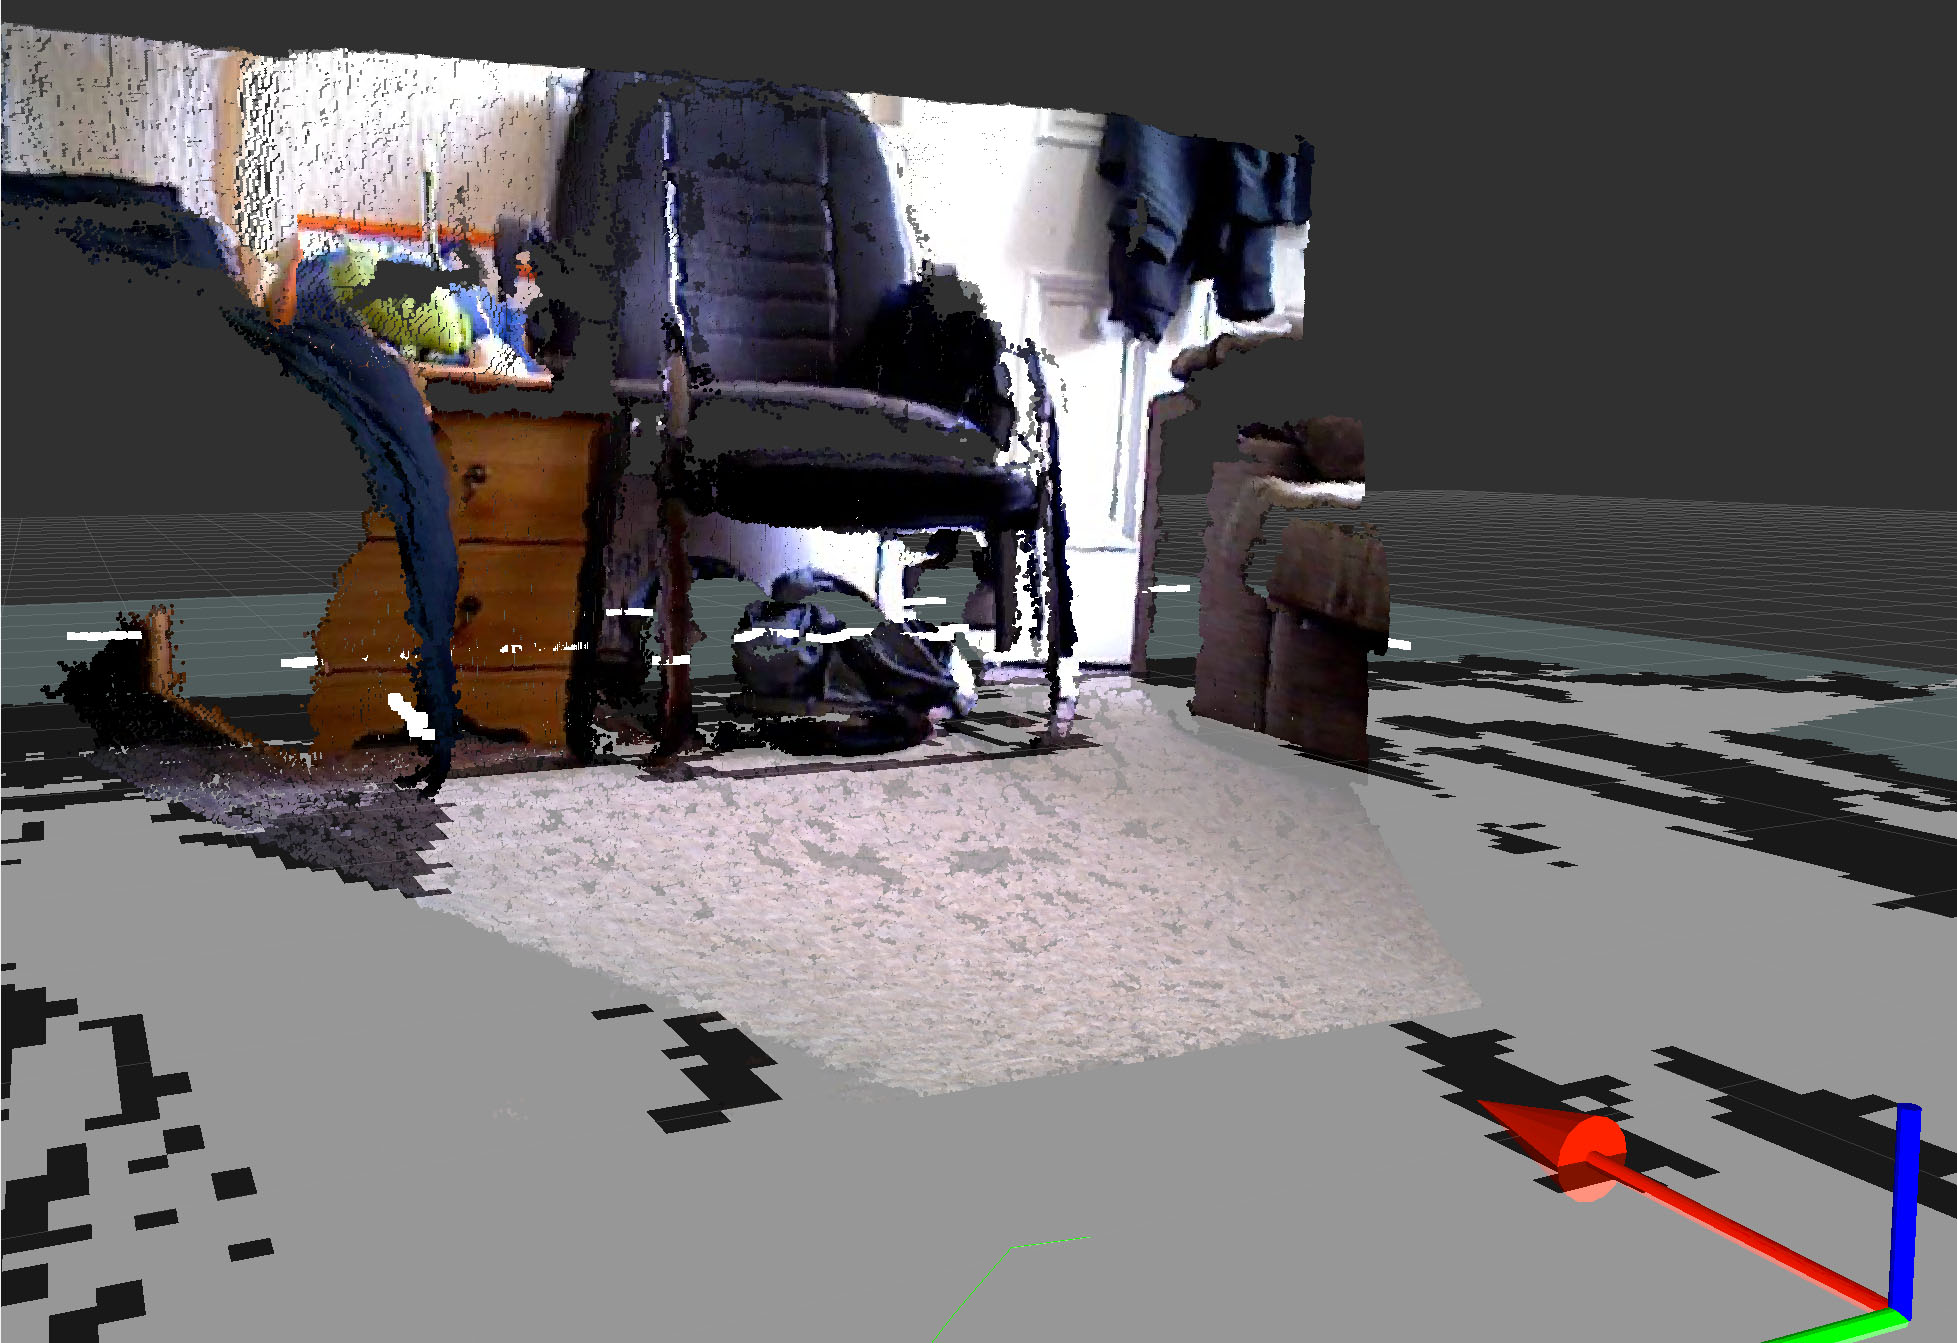
\includegraphics[width=10cm]{rgbd_pc2.jpg}
    \caption{Example point cloud output from the RGB-D camera mounted on top of the robot, as given by the \texttt{openni2\_camera} package, visualized using RViz. In this case, the points are projected into 3D space relative to the robot's position, and then coloured using the corresponding pixels on the RGB image.}
    \label{fig:rgbd_images2}
\end{figure}

The \texttt{openni2\_launch} package also publishes static TF transforms for the individual sensors on the camera, such that the slight difference in perspective can be corrected.

Camera calibration is also performed.

Understanding these package was rather troublesome, as both the wiki and GitHub pages documenting them were (and still are) completely blank. Instead, the documentation for a similar set of these packages for the first version of \emph{OpenNI}, named \texttt{openni\_launch}, was used \cite{ros_wiki_openni_launch}. Regardless, there was little difficulty in setting this package up.

\subsection{Servo Driver}

While there were already drivers available for the RGB-D sensor, the case was not the same for the servo controller. For this, a custom node had to be developed.

Python. pySerial.

Topics used so that any sending nodes don't need to queue or wait. Can cause conflicts however.

%%%%%%%%%%%%%%%%%%%%%%%%%%%%%%%%%%%%%%%%%%%%%%%%%%%%%%%%%%%%%%%%%%%%%%%%%%%%%%%%%%%%%%%%%%%%%%%%%%%%

\section{Locomotion}

Strictly, only joints 1 and 2 are necessary for a tripod gait. Joint 3 can be locked, perhaps as a single solid piece of material, such that a right angle is formed between the foot and leg sections. This provides a stable stance for the robot to balance upon as it pushes itself forward between each cycle.

\subsection{Limb Controller}

Splits limb into logical sections.

\subsection{Limb Calibration Tool}

Provides offsets.

\subsubsection{Usage}

Console app.

\subsection{Tripod Gait Walker}

Need diagrams.

\subsection{Joystick Controller}
Joy package, ez.

%%%%%%%%%%%%%%%%%%%%%%%%%%%%%%%%%%%%%%%%%%%%%%%%%%%%%%%%%%%%%%%%%%%%%%%%%%%%%%%%%%%%%%%%%%%%%%%%%%%%

\section{Sensing}

openni2 originally, ccny\_rgbd \cite{ccny_rgbd} provides some clean up features.

\subsection{Visual Odometry}

ccny\_rgbd \cite{ccny_rgbd} was used.

\subsection{Environment Mapping}

ocotomap

\subsubsection{Alternatives}

SLAM, but expects laser scan.

%%%%%%%%%%%%%%%%%%%%%%%%%%%%%%%%%%%%%%%%%%%%%%%%%%%%%%%%%%%%%%%%%%%%%%%%%%%%%%%%%%%%%%%%%%%%%%%%%%%%

\section{Navigation}

Built in stack.

\subsection{Path Planning}
